\section{Graphical Passwords}
\label{chapter:literatureReview}
  

\section*{Graphical Passwords} \label{sec:literaturegraphicalPasswords}

  Like text-based passwords schemes, graphical password schemes are also a knowledge-based authentication scheme, e.g. ``something you know'' that are described in the background theory. Since it all started around 1996, there have been many suggestions for graphical password schemes. When a new password scheme is proposed, there are several aspects of password that needs to be considered. A password scheme needs to be secure in terms of entropy, and it needs to be hard to guess and it also needs to be comfortable to use. This section will give a brief introduction to the history of research published on graphical passwords. This is important to know because each scheme is trying to improve different aspects of graphical password, giving us a detailed understanding of today's situation.

  Greg Blonder originally described the idea of graphical passwords in 1996 \cite{Blonder}. The graphical password scheme proposed was requiring the users to tap on a selection of points on a predefined image in order to pass the authentication process. This was just a proposal, and did not further explore the power of graphical passwords, nor analyzed the security aspects of the proposal.

  In 1999, Jermyn et al. \cite{Jermyn} suggested a new graphical password scheme called ``DAS'' (Draw-a-secret). Draw-A-Secret (DAS) was the first recall-based graphical password scheme proposed. The motivation for the graphical password scheme was that graphical input devices enables the user to decouple the position of inputs from the temporal order in which they occur, and shows that the decoupling can be used to generate passwords that have a larger and more memorable password space. In order to make a more memorable password, the research group argued that the DAS was more secure than text-based passwords because the users were able to remember longer and more complex passwords. After the DAS scheme was published, Dunphy and Yan \cite{BDAS} added an extra background image, called ``BDAS'', in order to encourage their users to make more complex passwords. 

  In Figure~\ref{fig:blonder} is showing the illustration from Blonder's patent of a graphical password scheme. Figure~\ref{fig:DAS} and Figure~\ref{fig:BDAS} is a figure of the DAS and BDAS respectively.

  \begin{figure}[H]
    \centering
    \subfigure[Proposal for a graphical password scheme\cite{Blonder}]{
      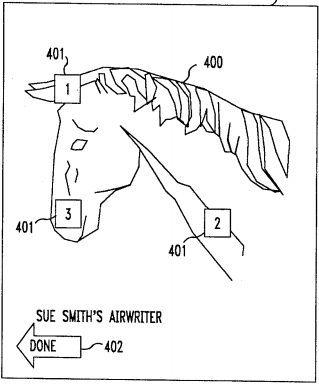
\includegraphics[width=0.30\textwidth]{pics/blonder.png}
      \label{fig:blonder}
    }
    \subfigure[DAS \cite{Jermyn}]{
      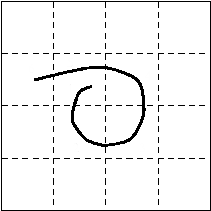
\includegraphics[width=0.30\textwidth]{pics/DAS.png}
      \label{fig:DAS}
    }
    \subfigure[BDAS \cite{BDAS}]{
      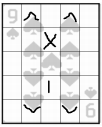
\includegraphics[width=0.30\textwidth]{pics/BDAS1.png}
      \label{fig:BDAS}
    }
  \end{figure}

  In 2000, Dhamija and Perrig \cite{DejaVu},created a new password scheme called ``Deja Vu''. The password scheme was based on the hash visualization technique \cite{HashVisualization}. The users are asked to select a sequence of images from a random set of images that are generated by the program. They wanted to make a graphical password scheme that solved some of the shortcomings with recall-based authentication like PIN's and text-based passwords. Deja vu should purely rely on recognition rather than recall, and it should be hard to write down and share the password with others. The randomly generated pictures based on the hash visualization technique makes it hard to share the password since the images is hard to recreate, but are easy to remember.

  ``Passfaces'' is a graphical password scheme developed by Real User Corporation that was founded in 2000 \cite{passface}. The authentication procedure allows the users to first select four images that are a visualization on human faces, and the user get authenticated by identifying their four faces. The scheme exploits the advantage that people are good at recognizing people, so when users choose the human faces, and they can recognize the characteristics of the faces.

  Figure~\ref{fig:DejaVu} is showing the Deja Vu password scheme using the hash visualization technique for generating images. Figure~\ref{fig:Passfaces} is showing the PassFaces scheme used on a smartphone. This is one of the few commercial graphical password schemes that are in use.

  \begin{figure}[H]
    \centering
    \ContinuedFloat
    \subfigure[DejaVu \cite{DejaVu}]{
      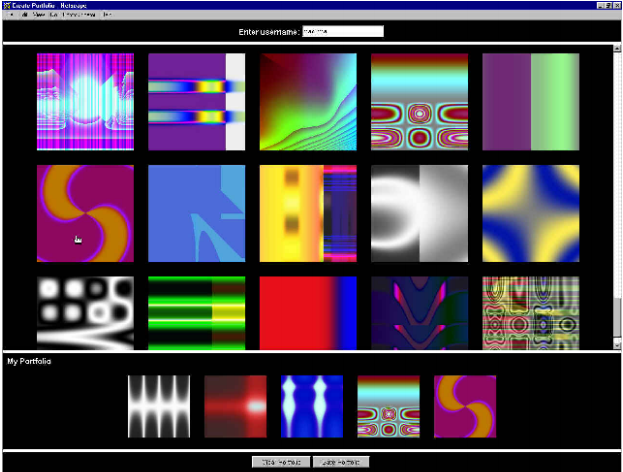
\includegraphics[scale=0.35]{pics/DejaVu1.png}
      \label{fig:DejaVu}
    }
    \subfigure[Passfaces \cite{passface}]{
      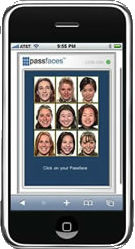
\includegraphics[scale=0.7]{pics/Passfaces.jpg}
      \label{fig:Passfaces}
    }
  \end{figure}

  In 2002, Goldberg et al. \cite{PassDoodle} tried to make a graphical password scheme that combines both text and images, named ``PassDoodle''. This is a graphical password combined with handwritten text. Their study concluded that users were able to remember complete doodle images as accurately as text-based passwords.

  In 2004, Davis et al. did a comparison of a light version of the ``PassFace'' and a new graphical password scheme called ``Story'' \cite{Davis}. The Story scheme is making the users choosing images making a story. The background for the scheme was to support their users of remembering their passwords by making a memorable story of images. The story that was made were needed to be recalled in the correct order. To support the memorability, users were instructed to construct a story mentally to connect the everyday images in the set.

  In 2005 Wiedenbeck et al. proposed a graphical password scheme called ``PassPoints'' \cite{Wiedenbeck2} that is an  extension of the Blonder's \cite{Blonder} idea by eliminating the boundaries and allowing arbitrary images to be used. They evaluated their password scheme by testing the scheme for human users. The results showed that PassPoint were a promising scheme with respect to memorability because of the low error rate and low clicking rate.
  The aim of this study was to get an understanding of how different images affected user performance in authentication with a graphical password scheme. The preliminary result showed suggested that images may support memorability in graphical password schemes.

  Figure~\ref{fig:story} is the Story scheme with images of faces and objects. Figure~\ref{fig:passpoints} is an image of the PassPoints scheme showing five selected points in the picture.

  \begin{figure}[H]
    \centering
    \ContinuedFloat
    \subfigure[Story \cite{Davis}]{
      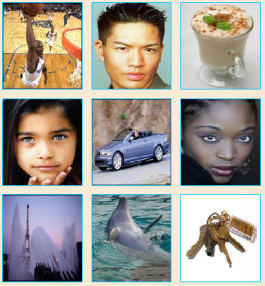
\includegraphics[scale=0.4]{pics/story.png}
      \label{fig:story}
    }
    \subfigure[PassPoints \cite{Wiedenbeck2}]{
      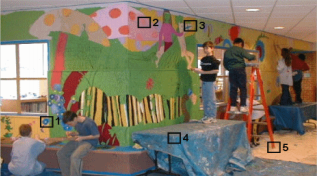
\includegraphics[scale=0.6]{pics/passpoint.png}
      \label{fig:passpoints}
    }  
  \end{figure}

  In 2006, a research wanted to address the problem with graphical passwords and the shoulder surfing problem. They called their password scheme ``Convex Hull Click'' (abbreviated CHC) \cite{Wiedenbeck}. The CHC that allows the user to prove knowledge of the graphical password in secure and insecure location because they made the scheme in a way that users do not directly click on their password images. This design makes it hard for attackers to perform shoulder surfing. In CHC, the windows show a list of small icons. In the authentication process, the user needs to recognize some minimum number of their chosen password images, or ``pass-icons'', out of a vast number of randomly placed icons. This step are presented in a sequence, and if the user responds correctly every time, the user pass the authentication. Figure~\ref{fig:chc} is a picture of the CHC password scheme with three selected icons.

  \begin{figure}[H]
    \centering
    \subfigure[CHC \cite{Wiedenbeck}]{
      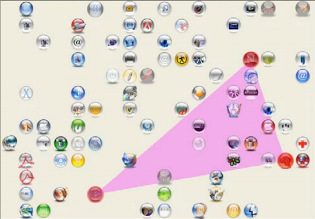
\includegraphics[scale=0.9]{pics/CHC.png}
      \label{fig:chc}
    }
  \end{figure}
  
  In 2007, Tao and Adams \cite{Tao}, created a new proposal for a new graphical password scheme called ``Pass-Go''. The Pass-Go scheme is inspired by the old Chinese game, Go, where users selects intersections on the grid to make their password. This was one of the first largest user studies on graphical passwords and was made in order to improve the usability of graphical passwords. They try to emphasize that the usability of a graphical password scheme will increase the memorability of graphical password, causing the password scheme to be more secure.
  Figure~\ref{fig:passgo} is an image of the Pass-Go grid used. 
  Graphical passwords are also implemented on mobile devices, like the ``Android Unlock Pattern'', that is a mini version of the ``Pass-Go'' deployed on Google Android smartphones. ``PatternLock'' is a similar system that are available for Blackberry. Rather than entering a four-digit PIN or a text-based password, the user enters a touch-drawn password on a $3\times3$ grid.

  Figure~\ref{fig:android} is the Android Unlock Pattern in use on a smartphone.

  \begin{figure}[H]
    \centering
    \ContinuedFloat
    \subfigure[Pass-go \cite{Tao}]{
      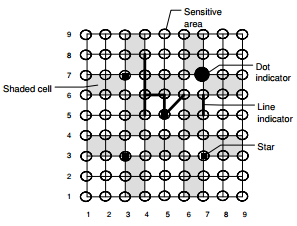
\includegraphics[scale=0.7]{pics/passgo.png}
      \label{fig:passgo}
    }
    \subfigure[Android Unlock Pattern]{
      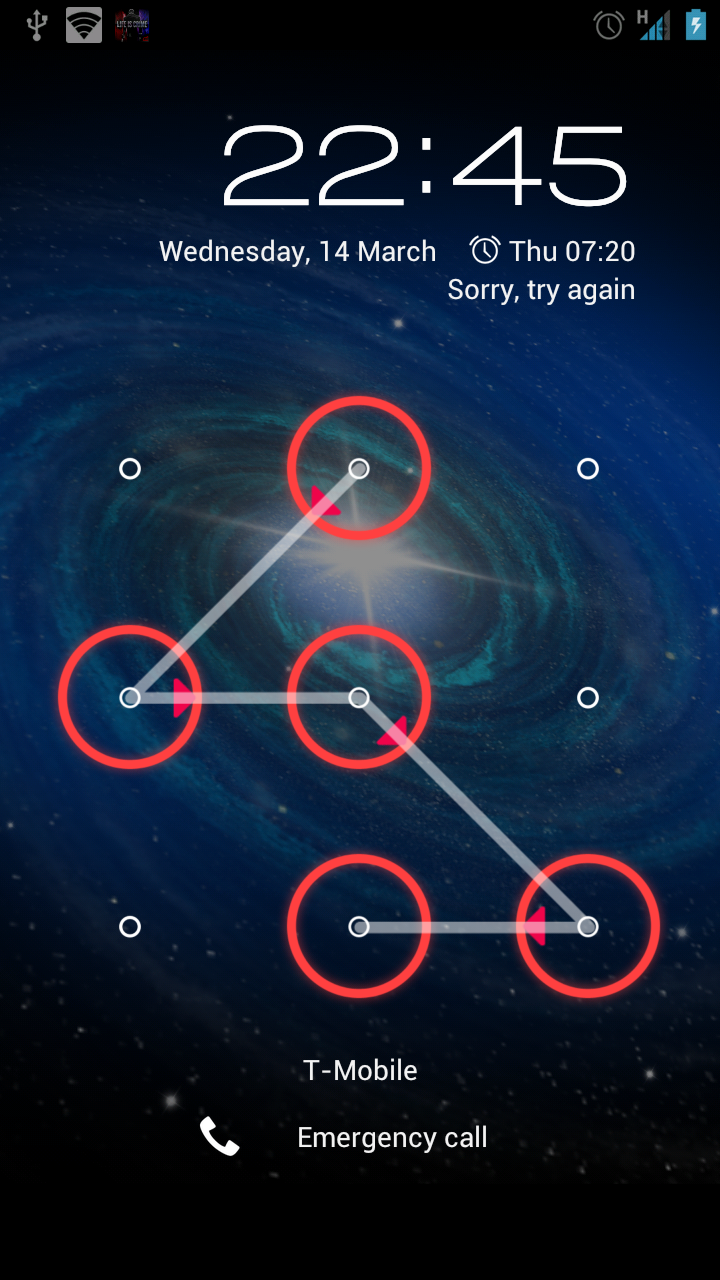
\includegraphics[scale=0.15]{pics/patternLock.png}
      \label{fig:android}
    }
  \end{figure}

  Graphical passwords are still not widely adopted, but there are still new graphical password scheme being proposed. Recently published graphical password schemes are GeoPass \cite{GeoPass} and Picassopass \cite{PicassoPass}. Geopass uses a digital map for the authentication phase, where the user chooses a particular location as their password. Picassopass is a graphical password scheme that are presenting a password using a dynamic layered combination of graphical elements. The users can make a story that assists the user in the recognition of the graphical elements.

  Figure~\ref{fig:geopass} and Figure~\ref{fig:PicassoPass} is the two new proposals for graphical authentication schemes, the Geopass and the Picassopass, respectively. 

  \begin{figure}[H]
    \centering
    \ContinuedFloat
    \subfigure[GeoPass \cite{GeoPass}]{
      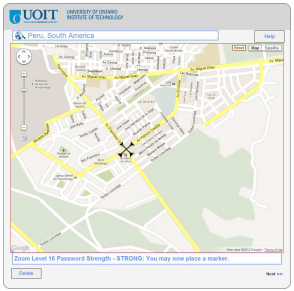
\includegraphics[scale=0.60]{pics/geopass.png}
      \label{fig:geopass}
    }
    \subfigure[PicassoPass \cite{PicassoPass}]{
      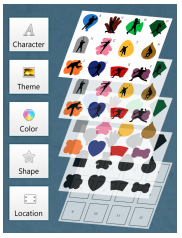
\includegraphics[scale=0.80]{pics/picassopass.png}
      \label{fig:PicassoPass}
    }
    \caption{Graphical password schemes}
  \end{figure}

  \clearpage
 \section{Evaluation of Graphical Password Schemes} \label{sec:evaluation}

  \begin{wrapfigure}{l}{0.4\textwidth}
    \vspace{-20pt}
    \begin{center}
      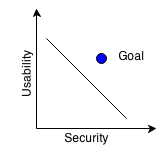
\includegraphics[scale=0.75]{pics/UsabilityVsSecurity.png}
    \end{center}
    \vspace{-20pt}
    \caption{Usability vs. Security}
    \vspace{-10pt}
    \label{fig:usabilitysecurity}
  \end{wrapfigure}

  Authentication with text-based passwords are a common approach, but it is well known that users often choose weaker passwords because of the limitations of recalling text-based passwords. Graphical passwords came as an alternative solution for overcoming the limitations of text-based passwords, and was inspired by researchers that showed that the graphical memory of humans is particularly well-suited to remember graphical information \cite{DeAngeli}. The problem with many graphical password schemes is that they often promise improved password memorability and thus usability, and at the same time improve the security \cite{Biddle}. The trade-off between usability and security is illustrated in Figure~\ref{fig:usabilitysecurity}. Because of the observed trade-off between usability and security, it is important to understand both the usability and security aspects when looking at different password schemes.

\subsection{Usability and Memorability} \label{sec:usability}

  \todo{Finne forskning som evaluerer grafiske password på usability and memorability}

  An interesting question to be asked is what classes of graphical password users find memorable. Based on cognitive studies of visual information, Oorschot and Thorpe \cite{Thorpe1} investigated the memorable password in the graphical password scheme DAS \cite{Jermyn}. They found that the were less or equal to the length of 8 on a 5$\times$5 grid. This results compared to textual passwords may offer greater security against dictionary attacks.

  If the number of possible pictures in a graphical password scheme is large enough, and the diversity of the of picture based passwords can be captured, it seems reasonable to argue that memorable password space of a graphical password scheme will be higher than text-based password schemes. This makes graphical passwords offering better resistance to dictionary attacks. When the proposal for the graphical password scheme ``Deja Vu'' was proposed, they did a user study that showed that 90\% of all participants succeeded in the authentication tests using Deja Vu while only about 70\% succeeded using passwords and PINS \cite{DejaVu}. This is an example that users tend to have a higher success rate remembering graphical password, rather than text-based passwords.

  One of the first graphical password schemes, ``DAS'' \cite{Jermyn}, offers a theoretical space that are comparable with text-based passwords. The results from research show that users tend to draw symmetric images with few pen strokes, and often place their drawings in the center of the grid. The ``Background Draw A Secret'' scheme (Abbreviated BDAS) \cite{BDAS} tried to avoid users placing their drawings in a predictable way. In BDAS, they added an additional background image. The attached background image resulted in a reduced amount of symmetry within the selected passwords, and supported the users to make longer passwords that were similarly memorable as for the ``DAS''. It remains still a problem that many of the research published on graphical passwords are performed with a pen and paper approach, raising a question about the validity of the results. One problem may be that many graphical passwords are not implemented, but only a theoretical suggestions. It remains much research on graphical passwords in their intended environment.

  Davis \cite{Davis} did a comparison of the memorability between the graphical password scheme ``Face'' (a light version of the ``PassFaces'') and ``Story''. This results reported that users had more difficulty remembering Story password (success rate of 85\%), mostly of the errors was introduced because they had to remember the correct sequence of the images.

  When looking at usability, we can evaluate the graphical layout of a graphical password scheme to see if the visual elements impacts the user's choice of passwords. Ullenbeck et al. \cite{Uellenbeck} looked at the Android Unlock patterns and investigated if a change in the graphical layout would impact the security. The Android Patten Lock is made on a 3$\times$3 grid of connected points. Instead, they rearranged the points in 4 different positions and analyzed collected data. The results showed that they managed to double the password space by rearranging the points and reduce the biases that are found in the original position of the nodes, but also introduce new ones. One of the rearrangements was a random approach. Unfortunately, this random arrangement of nodes looked like the mathematical ``delta'', so many people recognized the symbol. The random arrangement scored the worst entropy since many of the users chose the same pattern. They did not have several recognizable arrangements, but since people are good at recognizing and memorize patterns, it would not be surprisingly if they would find the same results in other rearrangements that was similar to a user known symbol.

  Wiedenbeck et al. \cite{Wiedenbeck1, Wiedenbeck2, Wiedenbeck3} conducted three lab-based user studies of the graphical password scheme ``PassPoint''. The results showed that the users needed an average time of 63 seconds in order to create their password, and an additional average time of 171 seconds in training time in order to remember the password. The login time took an average time of 9 and 19 seconds. This highlights important research on usability and memorability of a graphical password scheme. Some of the factors that make a password scheme to have high usability is deiced by average creation time, time to remember the password, as well as time used in the login phase. 

  \todo{Legge til forskning på usability av pass-go}

    
\subsection{Security} \label{sec:security}

  In knowledge-based authentication, e.g. ``something you know'' we classify attacks into two general categories: guessing and capturing attacks. In a guessing attack the attackers are able to search through the entire password space, or either predict the users passwords patterns in order to avoid searching through the whole passwords space (often referred to as a dictionary attack). This is often associated with the entropy of the password, because the lower the entropy it will be easier to make a successful attack. When talking about capturing attacks, the attackers can directly obtain the passwords by observing the authentication process. One of the known capturing attacks on graphical passwords is shoulder surfing because of its graphical visualization.

  Since a person needs to remember a password, it is normally to choose a password that are connected to you as a person in order to remember the password, causing the password to be biased. A bias can be explained as a prejudice in favor of or against one thing, person, or group compared with another, usually in a way that influence a person choice of action. Since psychological studies have recognized that the human brain have a superior memory for recognizing and recalling visual information, it support the statement that users are able to remember more complicated graphical password form a larger password space than a alphanumeric password. Logically the attacker then has to build a bigger and more complex dictionary, thus spend more time to achieve the same success rate as for textual passwords.

  The graphical password scheme DAS \cite{Jermyn} was evaluating the security of their password scheme. They highlighted that there are many factors that impacts the security of a password scheme, like the statement that the users do not use a uniform distribution of all possible passwords, using Klein's study \cite{UnixPasswords} as a argument. The fact that users do not pick passwords uniformly is not in itself a sufficient statement to make a guessing attack successful. They try to cover the possibility of an attacker making a successful attack by making their scheme complex, and the results showed that the generated passwords were significantly harder to crack in practice than textual passwords. The problem is that they used computer generated passwords that will not show real user-selected passwords. They did not analyze the security of the DAS including human factors and password biases that may influence the practical password space.

  There is a lack of analysis on graphical password on users choices in graphical passwords. Davis et al.\cite{Davis} evaluated the security of the ``PassFace'' graphical password scheme. They found that there was a bias that was introduced by the demographics of the users. The users tended to choose faces that they liked and could compare themselves to. The results showed that if you knew the gender and race of the user, you could perform a dictionary attack to guess user's passwords. If the gender of the user was known as male, then 10\% of the passwords can be easily guessed on the first or second attempt. Similarly, if the race of the user was known to be Asian and his/her gender is known, then 10\% of the worst passwords can be guessed within the first six attempts. The results indicated that the human passwords were heavily biased, and they stated that the graphical password scheme was insecure.

  Dirik et al. \cite{Dirik} conducted an experiment by modeling user choice in the graphical password scheme ``PassPoints''. The aim of this study was to test if it was possible to build a dictionary attack based on user's choice in clicking points. In this study, they predefined two different images with a different level of salient points. The results stated that they could recover 61\% of the user's passwords by searching through a smaller password space that was based on an analysis of collected click-points. The ``PassPoints'' scheme provides user-chosen password, but the aim of this study was to investigate if it was possible to predict users password in a dictionary attack. There was a slight difference in the two images that the researcher picked, where the image with less salient points was stated as insecure. Since the ``PassPoints'' scheme enables user-selected passwords, the security may rely on the selected image by the user, and not the actual scheme. The results of this research can not it selves state that the ``PassPoints'' scheme is insecure. It rather highlights the importance of considering the human factors in security because it may influence the overall security of a graphical password scheme. The same year another research group published \cite{Thorpe2} results on security of the ``Passpoints'', but using different approaches. They conducted a user studies to test if it was possible to make an offline attack as well as using an image-processing tool for simulating an offline attack on the same images that were used in the user studies. They provided empirical evidence that attractive points, e.g. hot-spots do exist in images. The results from the most efficient attack were generated by harvesting passwords from users to attack other targets. The probability of the guessing attack showed that 36\% of the passwords selected by users could be guessed within $2^{31}$ guesses and 12\% within $2^{16}$ guesses. The results from the offline attack using image-processing were slightly less efficient, but they still managed to prove that an offline attack is possible to use on graphical passwords.   

  \todo{Her må jeg ha med flere eksempler på forskning som fokuserer på angrep}

  In one of the first large-scale studies on the Android Pattern Lock \cite{Uellenbeck}, they stated that the entropy of patterns is lower than its theoretical entropy. The results of the study indicated that the security offered is less than the security of only three digits randomly assigned PIN for guessing 20\% of all passwords. In the same research, they made a Markov model based on collected passwords from users categorized as offensive and defensive patterns in their user study. The results showed that it was possible to guess user's choice in patterns. Within ten guesses, they could guess approximately 4\% of pattern in the category defensive patterns and approximately 7\% of the defensive patterns. When increasing the number of guesses to 30 attempts, they managed to guess approximately 9\% of the defensive patterns and approximately 19\% of the offensive patterns. If we look further into the Android Unlock Pattern, it have nearly 400.000 possible patterns and are from a theoretical point of view stronger than a 5-digit randomly assigned PIN. The researchers evaluation of user chosen patterns shows that they only have an estimated entropy slightly lower than a 3-digit randomly assigned PINs. Another interesting result is the memorable password space used, where about 10\% of all users use less than 190 patterns, while less than 300 patterns capture around 50\% of the whole test population. This shows that an empirical password space are not a representative number when quantifying the security of a password. We should rather look at the memorable password space, e.g. password that are used and memorized by users. The aim of this study was to close gap of lacking research on the practical password space on graphical passwords.

  A clever attacker would narrow down the password space and prioritize guesses to pictures that people are likely to choose. The images that are selected are liable to be the images that users are likely to recall. In order to understand how an attacker might take advantage of human password choices, psychological studies on humans visual memory are crucial to comprehend.. 

\clearpage
\section{Psychology and Human Factors} \label{sec:humanfactors}

  \begin{wrapfigure}{r}{0.35\textwidth}
    \vspace{-20pt}
    \begin{center}
      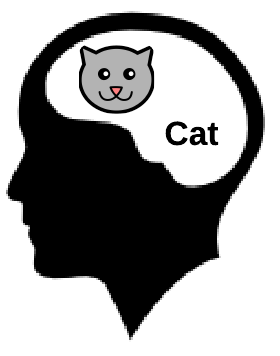
\includegraphics[scale=0.35]{pics/dualCoding.png}
    \end{center}
    \vspace{-20pt}
    \caption{Dual-Coding Theory}
    \vspace{-10pt}
    \label{fig:dualcoding}
  \end{wrapfigure}

  In many years, the field of psychology been an important in order to understand how humans interpret and remember different information. Psychology studies have recognized that the human brain have a superior memory for recognizing and recalling visual information rather than recognizing and recalling verbal or textual information \cite{DeAngeli}. One known theory is the ``dual-coding theory'' \cite{Biddle}, suggesting that verbal and non-verbal memory are processed and represented differently in human's mind. Text are verbal information that is represented symbolically, in contrast to non-verbal information like images that are mentally represented in a way that perceived concepts are assigned to a perceived meaning of what is directly observed. Both verbal and non-verbal information can be used when recalling information. For example, say a person have received stimulus of the concept ``cat'', both the image of a cat as well as the word ``cat'' (Figure~\ref{fig:dualcoding}). When a person is asked to recall the concept ``cat'', a person can retrieve the image or the word individually, or both simultaneously. If the word ``cat'' is remembered, the picture of the cat is not lost and can still be retrieved at a later point in time. The ability to code a stimulus in two different ways can increase humans ability to remember, in contrast to only code the stimulus in one way. In the background theory there are described three various categories of graphical passwords according to the memory task involved in remembering and entering the password, e.g. recall, recognition and cued recall.

  When it comes to humans and visual interpretation, studies support the idea that people recall symmetric images better than asymmetric images \cite{Attneave, French}. A particular interesting observation is that mirror symmetry carries a special status I the human memory \cite{Wagemans1}. An understanding of psychological studies on humans visual memory can help to build successful attacks against graphical passwords. If an attacker can successfully use the symmetric properties of graphical password schemes, then the security may be significantly less than if all passwords were equivalent probable.

  Humans do not only tend to choose symmetric passwords, but do also tend to be influenced by the graphical elements in a password scheme. A study on ``PassFace'' \cite{Davis} showed that there was a high bias in the password selection according to a user's gender and race. When they analyzed how each gender chooses their password, the most of the male and female participants chose female faces, and 60-70\% of the user chose a model over a typical female/male. They also looked at the race of the faces, where the results showed that almost all of the participant chose their own race. This research raises the question if it is possible to analyze user's choice in passwords based on the demographics of the user.

  A difference in graphical and text-based password schemes is that graphical passwords can use images with colors that may influence the user's choice in graphical passwords. In a user-study \cite{Thorpe2} on the image-based graphical password scheme ``PassPoints'' managed to see that different images were easier guessed than other pictures. When analyzing different images and visualizations, we can look at studies of gestalt psychology \cite{Wagemans2} that uses the gestalt principles to understand user's interpretation of the picture. One of the images that were the easiest to guess in the user-study was an image with cars in different positions in different colors. A possible explanation could be that humans seek to find a pattern that are easily remembered by using the principles of grouping, similarities of color, and similarity of size in image analysis.

  There are many studies on password based on psychology and human factors, but the graphical passwords schemes being analyzed do not look at the background of the users. Humans are different in terms of their demographics, like gender, age, and culture in their country. Analysis of people choices of graphical password based on user's background have not been looked further into in published research as based on this state of the art research. Since there is a lack of this on graphical password, we will take a look at people choices on text-based passwords based on human properties.

  Password habits may be different across different subpopulation in cause of different background or culture. In 2012 Joseph Bonneau released an analysis of 70 million passwords from Yahoo! \cite{Bonneau2}. The data is analyzed in terms of guessing rate by using a dictionary attack. The collected data contained 328 subpopulations. The results showed that there was no ``good'' populations from the gathered data, but there was a variation in the population. Demographically, the gender had a small effect on the guessing rate, but it showed that age tended to give effect where password strength increases across different age groups. The analysis also showed that language had a significant impact on the password strength where Indonesian-speaking users were among the weakest subpopulations, and in contrast the German and Korean-speaking users provided relatively stronger passwords.

  \todo{Legge til mer forskning}
  \todo{Legge til studier fra psykologi som kan forklare hvordan mennesker ser på sammensetningen av et bilde (cognitive studies)}
  

  \section{Graphical Passwords and Mobile Devices} \label{sec:mobiledevice}
  %Intro
  Users are not only dependent on remembering passwords across multiple web pages and systems, but do also need to remember passwords for our small mobile devices. The mobile phone have emerged as an excellent platform for graphical passwords because it is easier to input on touchscreen as a contrast to text-based passwords. Graphical passwords on mobile devices seem like a natural fit, as they often require direct manipulation of visual elements. In today's society, we are addicted to our mobile devices in our everyday life. Mobile devices are not just a communication tool for calling and texting, but also a valuable tool for daily tasks like doing our work, reading mail, pay our bills and keeping up with our social life. This trend makes our mobile devices vulnerable in terms of security. To avoid unwanted access, smartphones offer different locking mechanisms. The history of locking mechanisms was often a solution solely to prevent accidental use, while current mobile phones require protection in order to secure the potentially vast amount of private data that we keep on our smartphones. The situation of our rapid use of mobile phones, as well as it well-suited platform for graphical password, makes authentication on mobile devices an interesting field of study.

  When looking at mobile security it essential to be familiar with the magnitude of mobile phone usage. As of 2014, over 90\% of American adults owns a mobile phone, whereas 58\% of American adults owns a smartphone \cite{MobileUseage}. Another 34\% of the users used their phone mostly to go online instead of using other devices such as a desktop or laptop computer. This is numbers from USA, but it still provides insight information about the use of mobile phones today.

  % Awareness about the sensitivity of the data stored mobile phones
  As stated earlier, smartphone user's tends to store sensitive information on their phones, it is important to understand the relationship between the use of security features and users risk perceptions. One of the key security aspects on mobile phones that are important to understand is why people use or not use locking mechanisms on their smartphone. Engelman et al. \cite{Egelman} published a research paper in cooperation with Google on people's smartphone locking behavior and attitudes towards security of their smartphone data. They observed a strong correlation between the use of security features and risk perceptions. They reported that 33\% of the smartphone users were thinking about the locking mechanisms as too much of a hassle, while 26\% of the user's didn't think that someone would care about the information stored on their phone. Other reported results have covered that the 46.8\% of the participants agreed or fully agreed that unlocking their phone can be annoying. At the same time, 95.5\% of the users somewhat agreed or fully agreed that they liked the idea that their phone was protected \cite{habits3}. The study reported that 29\% did not lock their smartphones \cite{MobileUseage} while another research stated that among 35\% of mobile users do not lock their phone \cite{Bruggen}. The number may vary because of the background and experiences with security while the number remains quite high. This highlights that the users want to be secure, but there might be a trade-off between the time used to unlock the smartphone vs. the security risk. 

  % The time used on unlocking the phone
  In terms of security, it is interesting to look at the use of mobile devices and look at the locking habits among users on mobile devices. It is known that services that are rapidly used have weaker password because of the overhead the user needs to spend on typing their password. In 2014 a group of researchers published a field study of smartphone (un)locking behavior \cite{habits3}. Some of the problems with smartphone users tends to be their rapid use of their phone. When the device is rapidly used, it results in much time unlocking their phone between every use. In the study they found that there was a significant overhead in the time used for unlocking their phone, where the users participated in the field study used 2.9\% (9\% in the worst case) of their time unlocking their smartphone.

  It is stated that many users use their smartphones to perform tasks that involve utilization and storage of sensitive data. Smartphones in use today do not require their users to have a locking mechanism on their smartphone. It is well known that users tends to choose the easiest way out and may result in the choice of not having any locking mechanism at all. Based on the outcome of the overhead in time used for unlocking their phone, the result may be to take the easiest way out by ignoring the vulnerability of not using a locking mechanism at all. It has been discovered that over 40\% of the users only used a basic ``slide-to-unlock'' mechanism on their smartphone, as well as over 16\% did not use any locking mechanisms at all \cite{habits3}. This highlights an important bad habit among mobile users. What happens if your mobile is stolen? A loss of a mobile phone is not just the cost of replacing the phone, but also a loss of sensitive data. If the wrong persons find the phone, the sensitive data on the phone may be lost and used for unintended purposes. A 2012 report from Pew Internet estimated that nearly a third of mobile users have had their device stolen or lost \cite{StolenLost}. It is interesting to comparing people's locking behavior towards phones that are stolen or lost. The same report also stated that 12\% of cell owners say that another person have accessed their phone, making the owners feel that their privacy have been exposed to the public.

  Besides losing a physical device, what consequences are users exposed to? One point of attack is to get access to a people's email. If you can grant access to someone's email, you probably can get access to a lot more. In a study reported that all of their interview participants had their email account automatically logged in, as well as 31\% of them did not use any locking mechanism at all \cite{Egelman}. The same research group investigated how much information you could gain from getting access to a person email account. The results showed that both users with or without locking mechanisms found sensitive information in their email account like SSN, Bank Account Number, Email Password and Home Address.

  One of the traditional password schemes on smartphones is the Android Unlock pattern. It is a graphical password scheme that have been shown to have biases when the password is user-chosen. A research group did one of the first large-scale user study on the security of the Android Unlock Patterns in order to quantify its security \cite{Uellenbeck}. They analyze the biases introduced in the pattern making process and added changes to the scheme in order to avoid the known biases in the password scheme. The researchers found that there is a high bias in the pattern selection process, e.g. the upper left corner and three-point long straight lines are very typical selection strategies. If the patterns were uniformly chosen, the probability of starting in at any point should be 11\%. The results showed that there was a strong bias to the starting point towards the corners. If the points were uniformly chosen, the probability for all four corners should be 44\%, but the results showed that the probability is close to 75\% in the pen-and-paper study. In contrast to this, the center point, the right, the upper, and the lower center points only get a probability of 14\% based on the results. Other results from the pen-and-paper study found that the average pattern length was 5.63 (with a standard deviation of 1.5). By looking further into the pattern length chosen by users, this is not a surprisingly result because this seems quite familiar with restriction of the Android Pattern Lock that requires the users to make a pattern of at least 4 connected points. As stated earlier, users tend to take the easiest way out, making users choose short patterns that are easy to remember and type. Besides the pen-and-paper study, there was also conducted a user study that also showed a high bias towards the upper-left corner that had the bias of 43\% in the user study, and 38\% in the pen-and-paper study. This is supporting the researchers claim that users tend to choose less secure patterns ``in the wild''.
  
  The way that the mobile phone is held, the size of the screen may also impact the way that people write their passwords, but this may need further research to answer.

  
